% Lead: Leanne, Reviewed by Gregory, Wil, Adam.
\section{Rubin Science Platform}
\label{sec:data_services}

The \gls{RSP} \citep{LSE-319,DMTN-212} is a powerful, cloud-based environment for scientific research and analysis of petascale-scale astronomical survey data.
It serves as the primary interface for scientists to access, visualize, and conduct next-to-the-data analysis of Rubin and \gls{LSST} data.
The  \gls{RSP} is designed around a  ``bring the compute to the data'' principle, eliminating the need for users to download massive datasets.
Although \gls{DP1} is comparable in size (\sizeinbytes) to existing survey datasets, future \gls{LSST} datasets will be larger and more complex, making it crucial to co-locate data and analysis for effective scientific discovery.

The \gls{RSP} provides users with access to data and services through three distinct user-facing Aspects: a \emph{Portal}, which facilitates interactive exploration of the data; a JupyterLab-based \emph{Notebook} environment for data analysis using Python; and an extensive set of \emph{\glspl{API}} that enable programmatic access to both data and services.
The three Aspects are designed to be fully integrated, enabling seamless workflows across the \gls{RSP}.
The data products described in \secref{sec:data_products} are accessible via all three Aspects, and the system facilitates operations such as starting a query in one Aspect and retrieving its results in another.
\figref{fig:rsp_landing_page} shows the Rubin \gls{Science Platform} landing page in the Google cloud.
\begin{figure}[htb!]
\centering
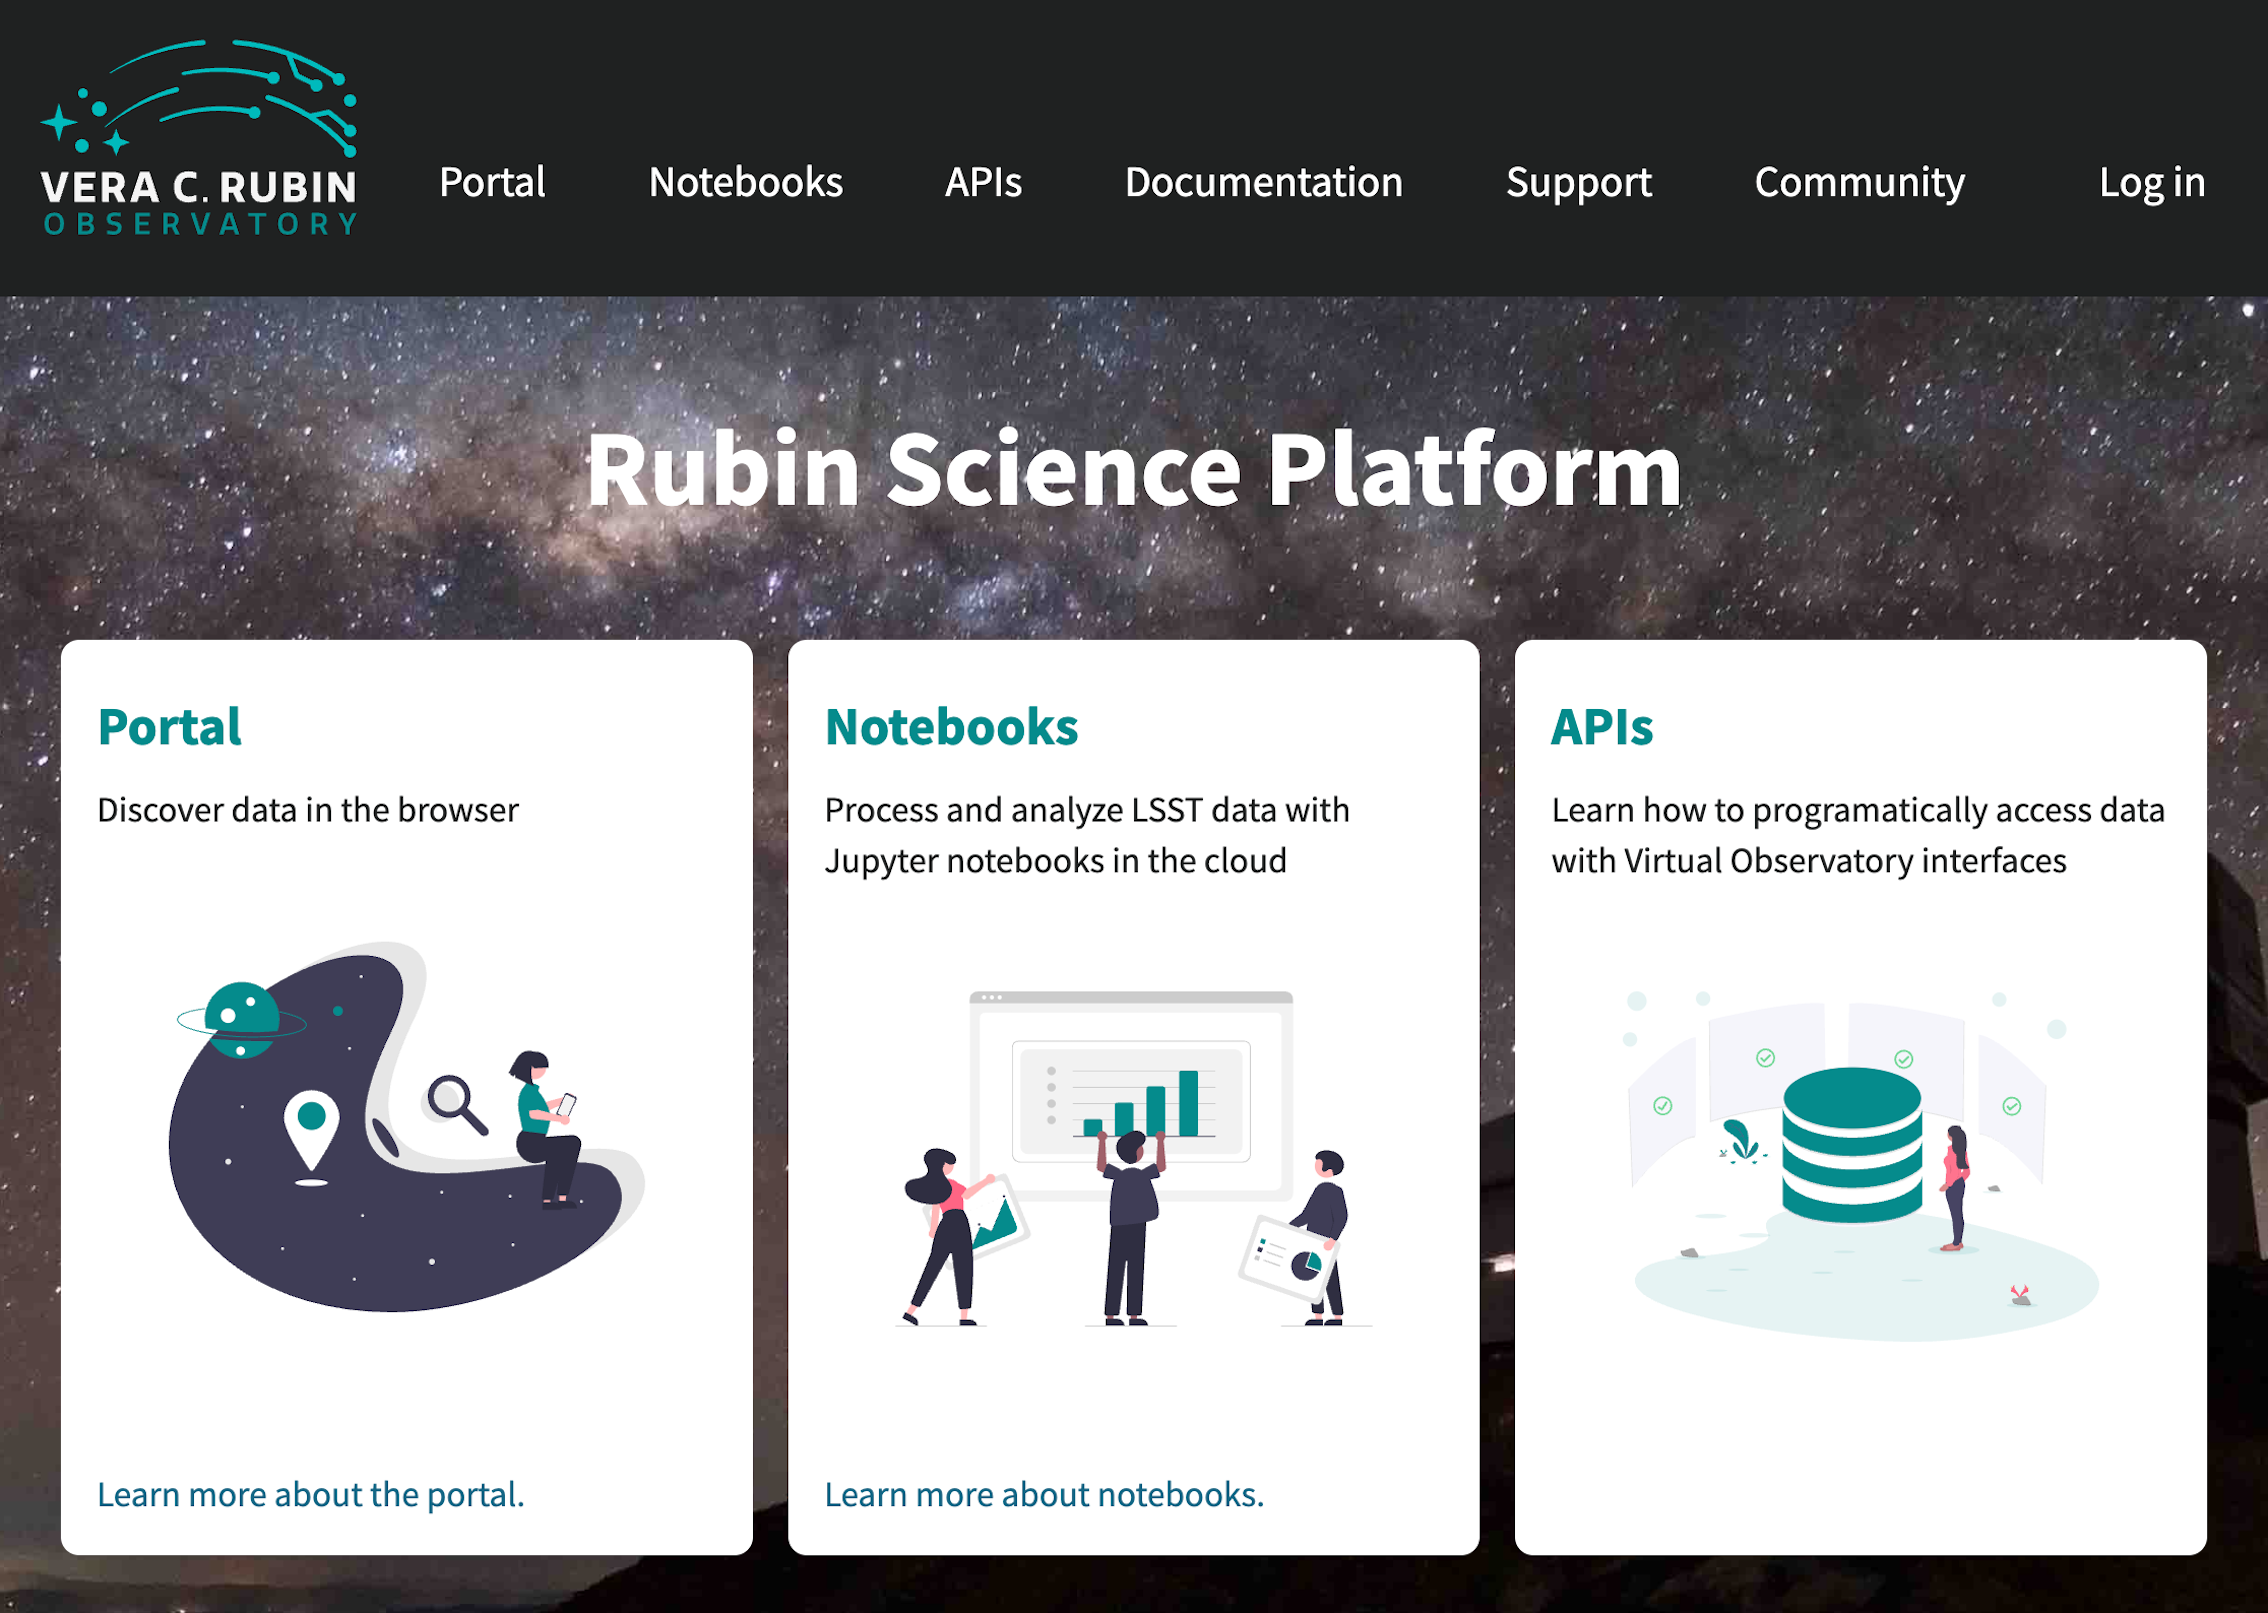
\includegraphics[width=0.98\linewidth]{data_access/rsp_landing_page.png}
\caption{The Rubin \gls{Science Platform} landing page showing the thress Aspects as well as links to documentation and support information.}
\label{fig:rsp_landing_page}
\vspace{0.1cm}
\end{figure}

The \gls{RSP} is supported by a number of back-end services, including databases, files, and batch computing.
Support for collaborative work through shared workspaces is also included in the \gls{RSP}.

A preview of the \gls{RSP} was launched on Google Cloud in 2022, operating under a shared-risk model to support \href{https://dp0.lsst.io/}{Data Preview 0} \citep{2024ASPC..535..227O}. This allowed the community to test the platform, begin preparations  for science, and provide valuable feedback to inform ongoing development.
It was the first time an astronomical research environment was hosted in a \gls{cloud} environment.
The DP1 release brings major updates to \gls{RSP} services, enhancing scientific analysis capabilities.
The \gls{RSP} remains under active development, with incremental improvements being rolled out as they mature.
During the Rubin Early Science Phase, the \gls{RSP} will continue to operate under a shared-risk model.
This section outlines the RSP functionality available at the time of the DP1 release and provides an overview of planned future capabilities.

% Section reviewed by Adam
\subsection{Rubin Data Access Center
\label{ssec:usdac}}
The Rubin USDAC utilizes a novel hybrid on-premises-\gls{cloud} architecture, which combines on-premises infrastructure at the \gls{USDF} at SLAC with flexible and scalable resources in the Google \gls{cloud}.
This architecture has been deployed and tested using the larger simulated data set of DP0.2 \citep{2024SPIE13101E..2BO}.

In this hybrid model, user-facing services are deployed in the \gls{cloud} to support
dynamic scaling in response to user demand and to simplify the provisioning and management of large numbers of science user accounts.
The majority of the static data products described in \secref{sec:data_products} are stored on-premises at the \gls{USDF} to benefit from cost-effective mass storage and close integration with Rubin data processing infrastructure, also located at the \gls{USDF}.
For imaging data, the Data Butler (\secref{sssec:data_butler}) provides the interface between the \gls{cloud}-based users and data services, and the on-premises data.
For catalog data, a \gls{cloud}-based \gls{TAP} client (\secref{sssec:ivoa_services}) submits queries to the on-premises \gls{Qserv} database cluster (\secref{ssec:databases}) and retrieves the results.
In the initial DP1 deployment, catalog data is hosted at the \gls{USDF} while image data is stored in the cloud.
The full hybrid model will be rolled out and further tested following the release of \gls{DP1}.

The RSP features a single-sign-on authentication and authorization system to provide secure access for Rubin data rights holders \citep{rdo-013}

\subsection{API Aspect
\label{ssec:rsp_api}}
The \gls{API} Aspect provides a comprehensive set of user-facing interfaces for programmatic access to the \gls{DP1} data products, through both \gls{IVOA}-compliant services and the Rubin Data Butler. IVOA services enable standard queries and integration with existing tools, while the Butler facilitates advanced data processing within the \gls{LSST Science Pipelines}.

At the time of the \gls{DP1} release, some \gls{IVOA} services are unavailable, and certain data products are only accessible via the Butler.
This section provides an overview of the available \gls{IVOA} services and Butler access.

% IVOA services
\subsubsection{IVOA Services
\label{sssec:ivoa_services}}

Rubin has adopted a \gls{VO}-first design philosophy, prioritizing compliance with \gls{IVOA} standard interfaces to foster interoperability, standardization, and collaboration.
In cases where standardized protocols have yet to be established, additional services have been introduced to complement these efforts.
This approach ensures that the RSP can be seamlessly integrated with community-standard tools such as TOPCAT \citep{2011ascl.soft01010T} and Aladin \citep{2000A&AS..143...33B, 2014ASPC..485..277B, 2022ASPC..532....7B}, as well as libraries such as  PyVO \citep{2014ascl.soft02004G}.

The user-facing \glspl{API} are also used internally within the \gls{RSP}, creating a unified design that ensures consistent and reproducible workflows across all three Aspects.
This reduces code duplication, simplifies maintenance, and ensures all users, both internal and external, access data in the same way.
For example, an \gls{ADQL} query on the \gls{Object} catalog via TAP yields identical results whether run from the Portal, Notebook, or an external client.

The following \gls{IVOA} services are available at the time of the DP1 release:
\begin{itemize}
\vspace{0.1cm}
\item \textbf{Table Access Protocol (TAP) Service}: A TAP service \citep{2019ivoa.spec.0927D} enables queries of catalog data via the IVOA-standard \gls{ADQL}, a dialect of SQL92 with spherical geometry extensions.
The main \gls{TAP} service for \gls{DP1} runs on the Rubin-developed \gls{Qserv} database (\S~\ref{ssec:databases}), which hosts the core science tables described in \secref{ssec:catalogs}, as well as the Visit database.
It also provides image metadata in the IVOA ObsCore format via the standard \texttt{ivoa.ObsCore} table, making it an ``ObsTAP'' service \citep[ObsTAP;][]{2017ivoa.spec.0509L}.
The TAP service is based on the \gls{CADC}'s open-source Java TAP implementation\footnote{https://github.com/opencadc/tap}, modified for the exact query language accepted by Qserv.
It currently supports a large subset of ADQL, with limitations documented in the data release materials (see \secref{ssec:documentation}) and exposed via the TAP \textbf{capabilities} endpoint where possible. \

The TAP service provides metadata annotations consistent with the standard, including table and column descriptions, indications of foreign-key relationships between tables, and column metadata such as units and \gls{IVOA} Unified Content Descriptors (UCDs).

% Image Services
\vspace{0.1cm}
\item \textbf{Image Access Services}: Rubin image access services are compliant with \gls{IVOA} SIAv2 \citep[Simple Image Access Protocol, version 2;][]{2025arXiv250100544J,2015ivoa.spec.1223D}
for discovering and accessing astronomical images based on \gls{metadata}.
For example, querying for all images in a given band over a particular sky region observed during a given period.
SIAv2 is a \gls{REST}-based protocol that supports the discovery and retrieval of image data.
%e.g. \url{https://<rubin-sia-service-url>?POS=180.0,0.0&SIZE=0.01}
Users identify an image or observation of interest and query the service.
The result set includes \gls{metadata} about the image, such as the sky position, time, or band, and a data access URL, which includes an IVOA Identifier uniquely identifying the dataset \citep{DMTN-302}, allowing the dataset to be retrieved or a cutout requested via \gls{SODA}.

% Image cutout services
\vspace{0.1cm}
\item \textbf{Image Cutout Service}: The Rubin Cutout Service \citep{SQR-063, SQR-093} is based on the  \gls{IVOA} SODA \citep[Server-side Operations for Data Access;][]{2017ivoa.spec.0517B}.
Users submit requests specifying sky coordinates and the cutout size as the radius from the coordinates, and the  service performs the operation on the full image and returns a result set.
% For a YxY cutout, the typical size of the returned result set is <X>
For \gls{DP1}, The  cutout service is a single cutout service only where N cutout requests will require N independent synchronous calls.
We expect some form of bulk cutout service by mid 2026, approximately contemporaneously with \gls{DP2}

% HIPS
\vspace{0.1cm}
\item \textbf{HiPS Data Service}: An authenticated \gls{HiPS}
%\footnote{HiPS is an IVOA standard for multi-resolution tiled image data.}
\citep{2017ivoa.spec.0519F}
%\citep[Hierarchical Progressive Surveys;][]{2017ivoa.spec.0519F}
data service for seamless pan-and-zoom access to large-scale co-adds.
It supports fast interactive progressive image exploration at a range of resolutions.

% WebDAV
\vspace{0.1cm}
\item \textbf{WebDAV}: A \gls{WebDav} service is provided to enable users to remotely manage, edit, and organize files and directories on the \gls{RSP} as if they were local files on their own computer. This is especially useful for local development.
\end{itemize}

%%%%% Data Butler
\subsubsection{Data Butler
\label{sssec:data_butler}}

The Rubin Data Butler \citep{2022SPIE12189E..11J,2023arXiv230303313L},  is a high-level interface designed to facilitate seamless access to data for both users and software systems.
This includes managing storage formats, physical locations, data staging, and database mappings.
A \gls{Butler} repository contains two components:
\begin{itemize}
    \item the \emph{Data Store}: A physical storage system for datasets, e.g., a \gls{POSIX} file system or S3 object store; and
    \item the \emph{Registry}: An \gls{SQL}-compatible database that stores metadata about the datasets in the data store, see \secref{sssec:butler_registry}.
\end{itemize}
% Current plan is for DP1 image data to be cloud-hosted for the initial release and then transition to USDF back-end once we get through the initial surge.
For DP1, the Butler repository is hosted in the Google Cloud, using an \gls{S3}-compatible store for datasets and AlloyDB, a PostgreSQL-compatible database, for the registry.

In the context of the \gls{Butler}, a \emph{dataset} refers to a unique data product, such as an image, catalog or map, generated by the observatory or processing pipelines
Datasets belong to one of the various types of data products, described in \secref{sec:data_products}.
The \gls{Butler} ensures that each dataset is uniquely identifiable by a combination of three pieces of information: a data coordinate, a dataset type, and a run collection.
For example, a dataset that represents a single raw image with detector 8 during the on-sky campaign on the night starting 2024-11-11 in the $i$ band with exposure ID 2024111100074 would be represented as  \texttt{dataId={'exposure':2024111100074, 'band':'i', 'instrument':'LSSTComCam'}} and is associated with the \texttt{raw} DatasetType.
For a deep coadd on a \gls{patch} of sky in the Seagull field, there would be no exposure dimensions and would instead the tract, \gls{patch} and band would be specified as  \texttt{dataId={'tract':7850, 'patch': 6, 'band':'g', 'instrument':'LSSTComCam', skymap='lsst\_cells\_v1'}} and is associated with the \texttt{deep\_coadd} DatasetType.

\begin{deluxetable}{lcc}
\tablecaption{Simple Test Table\label{tab:test} 
\label{tab:dp1_dimensions}}
\tablehead{
  \colhead{Name} & 
  \colhead{RA (deg)} & 
  \colhead{Dec (deg)}
}
\startdata
Star A & 12.345 & -45.678 \\
Star B & 98.765 & +32.100 \\
Star C & 210.123 & -0.456 \\
\enddata
\end{deluxetable}

The data coordinate is used to locate a dataset in multi-dimensional space, where dimensions are defined in terms of scientifically meaningful concepts, such as instrument, visit, detector or band.
For example, a calibrated single-visit image (\secref{ssec:science_images}) has dimensions including band, instrument, and detector.
In contrast, the visit table (\secref{ssec:catalogs}), a catalog of all calibrated single-epoch visits in \gls{DP1}, has only the instrument dimension.
The main dimensions used in \gls{DP1} are listed, together with a brief description, in \tabref{tab:dp1_dimensions}.
To determine which dimensions are relevant for a specific dataset, the \gls{Butler} defines dataset types, which associate each dataset with its specific set of relevant dimensions, as well as the associated Python type representing the dataset.
The dataset type defines the kind of data a dataset represents.
For example, a raw image  (\texttt{raw}), a processed catalog (\texttt{object\_forced\_source}), or a \gls{sky map} (\texttt{skyMap}).

\tabref{tab:butlerdatasets} lists all the dataset types available via the Butler in DP1, together with the dimensions needed to uniquely identify a specific dataset and the number of unique datasets of each type. It is important to highlight a key difference between accessing catalog data via the \gls{TAP} service versus the Butler. While the \gls{TAP} service contains entire catalogs, many of the same catalogs in the Butler are split into multiple separate catalogs. This is partly due to how these catalogs are generated, but also because of the way data is stored within and retrieved from the Butler repository -- it is inefficient to retrieve the entire \texttt{Source} catalog, for example, from the file system. Instead, because the \texttt{Source} catalog contains data for sources detected in the \texttt{visit\_image}s, there is one \texttt{Source} catalog in the Butler for each \texttt{visit\_image}. Similarly, there is one \texttt{Object} catalog for each \texttt{deep\_coadd}. All the catalogs described in \secref{ssec:catalogs}, aside from the \texttt{CcdVisit}, \texttt{SSObject}, \texttt{SSSource}, and \texttt{Calibration} catalogs, are split within the Butler.

%%%%% This table is auto generated from data, DO NOT EDIT
\setlength{\tabcolsep}{6pt}  % default is 6pt
\begin{deluxetable}{llcc}
\tablecaption{The name and number of each type of data product in the Butler and the dimensions required to identify a specific dataset.
\label{tab:butlerdatasets} }

\tablehead{
  \textbf{Data Product} & 
  \textbf{Name in Butler} & 
  \textbf{Required Dimensions} & 
  \textbf{Number in DP1}\
}
\startdata
\texttt{raw}&\texttt{raw}&instrument, detector, exposure&16125\\
\texttt{visit\_image}&\texttt{visit\_image}&instrument, detector, visit&15972\\
\texttt{deep\_coadd}&\texttt{deep\_coadd}&band, skymap, tract, patch&2644\\
\texttt{template\_coadd}&\texttt{template\_coadd}&band, skymap, tract, patch&2730\\
\texttt{difference\_image}&\texttt{difference\_image}&instrument, detector, visit&15972\\
\texttt{Source}&\texttt{source}&instrument, visit&1786\\
\texttt{Object}&\texttt{object}&skymap, tract&29\\
\texttt{ForcedSource}&\texttt{object\_forced\_source}&skymap, tract, patch&636\\
\texttt{DiaSource}&\texttt{dia\_source}&skymap, tract&25\\
\texttt{DiaObject}&\texttt{dia\_object}&skymap, tract&25\\
\texttt{ForcedSourceOnDiaObject}&\texttt{dia\_object\_forced\_source}&skymap, tract, patch&597\\
\texttt{CCDVisit}&\texttt{visit\_detector\_table}&instrument&1\\
\texttt{SSObject}&\texttt{ss\_object}&--&1\\
\texttt{SSSource}&\texttt{ss\_source}&--&1\\
\texttt{Visit}&\texttt{visit\_table}&instrument&1\\
\enddata
\end{deluxetable}


A dataset is associated with one or more \emph{Run Collections}; logical groupings of  datasets within the \gls{Butler} system that were created or processed together by the same batch operation.
Collections allow multiple datasets with the same data coordinate to coexist without conflict.
Run Collections support flexible, parallel processing by enabling repeated analyses of the same input data using different configurations.

For \gls{DP1}, a subset of the consolidated database contents (\secref{sssec:consdb}) is accessible through the Data Butler. However, not all metadata from the \texttt{Visit} table (\secref{ssec:metadata}) is available.
The \gls{DP1} Butler is read-only; a writeable Butler is expected by mid-2026, around the time of \gls{DP2}.

\subsubsection{Remote Programmatic Access
\label{sssec:remote_api}}
The Rubin \gls{RSP} \gls{API} can be accessed from a local system by data rights holders outside of the \gls{RSP}, by creating a user security token. This token can then be used as a bearer token for \gls{API} calls to the \gls{RSP} TAP service.
This capability is especially useful for remote data analysis using tools such as \gls{TOPCAT}, as well as enabling third-party systems (e.g., Community Alert Brokers) to access Rubin data. Additionally, it supports remote development with local IDEs, allowing for more flexible workflows and integration with external systems.

% Portal
\subsection{Portal Aspect
\label{ssec:rsp_portal}}
The Portal Aspect provides an interactive environment for exploratory data discovery, query, filtering, and visualization of both image and catalog data,  without requiring programming experience.

It enables users to search, visualize, and interact with large datasets through tools for catalog queries, image browsing, time series inspection, and cross-matching.
The Portal is designed to support both exploratory data access and detailed scientific investigation.

The Portal is built on \gls{Firefly} \citep{2019ASPC..521...32W}, a powerful web application framework developed by IPAC (Infrared Processing and Analysis Center).
\gls{Firefly} provides interactive capabilities such as customizable table views, image overlays, multi-panel visualizations, and linked displays between catalogs and images.
Through \gls{Firefly}, the Portal delivers a responsive and intuitive user experience, allowing users to analyze data visually while maintaining access to underlying metadata and query controls.
\begin{figure}[htb]
\centering
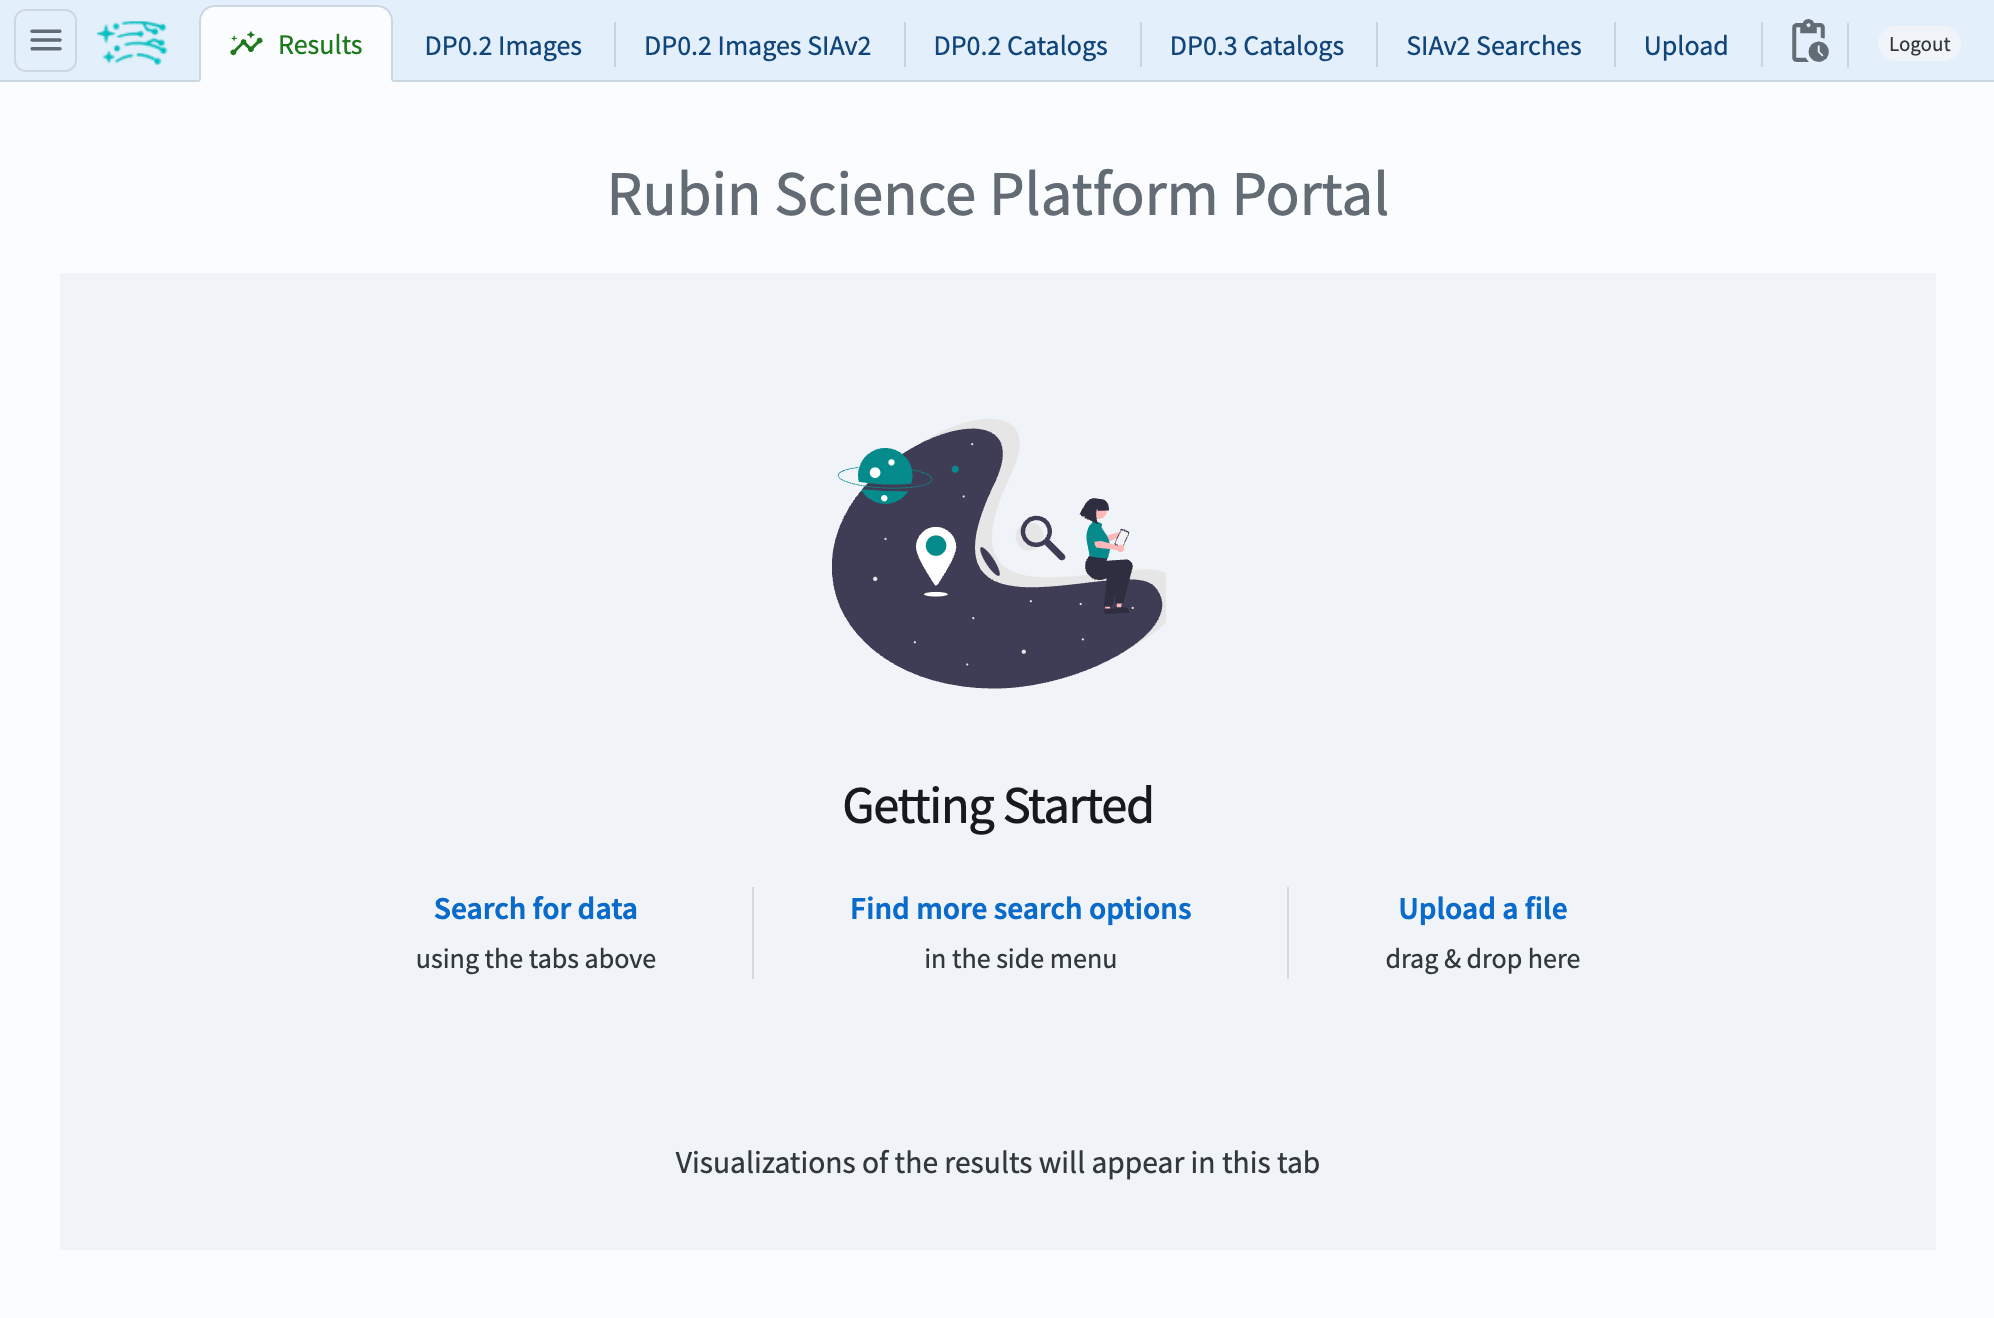
\includegraphics[width=0.98\linewidth]{data_access/rsp_portal_light.png}
\caption{The Rubin \gls{Science Platform} Portal Aspect}
% \gregory{Replace with a real DP1 image}
\label{fig:rsp_portal}
\end{figure}

\subsection{Notebook Aspect
\label{subsec:notebook}}
The Notebook Aspect provides an interactive, web-based environment built on Jupyter Notebooks, enabling users to write and execute Python code directly on Rubin and \gls{LSST} data without downloading it locally.
It offers programmatic access to Rubin and LSST data products, allowing users to query and retrieve datasets, manipulate and display images, compute derived properties, plot results, and reprocess data using the \gls{LSST Science Pipelines} (\secref{ssec:pipelines}).
The environment comes pre-installed with the pipelines and a broad set of widely used astronomical \gls{software} tools, supporting immediate and flexible data analysis.

\subsection{Databases
\label{ssec:databases}}
The user-facing Aspects of the \gls{RSP} are supported by several backend databases that store catalog data products, image metadata, and other derived datasets.
The \gls{schema} for DP1 and other Rubin databases is available online at \url{https://sdm-schemas.lsst.io}.

% Qserv -- Done
% Reviewed and approved by Fritz M.
% DP1 qserv catalog data will be hosted from SLAC from day 1.
\subsubsection{Qserv
\label{sssec:qserv}}
The final 10-year \gls{LSST} catalog is expected to reach \tenyearcatalogsize and contain measurements for billions of stars and galaxies across trillions of detections.
To support efficient storage, querying, and analysis of this dataset,  Rubin Observatory developed Qserv \citep{Wang:2011:QDS:2063348.2063364, C15_adassxxxii} -- a scalable, parallel, distributed SQL database system.
\gls{Qserv} partitions data over approximately equal-area regions of the celestial sphere, replicates data to ensure resilience and high availability, and uses shared scanning to reduce overall I/O load.
It also supports a package of scientific user-defined functions (SciSQL: \url{https://smonkewitz.github.io/scisql/}) simplifying complex queries involving spherical geometry, statistics, and photometry.
\gls{Qserv} is built on robust production-quality components, including MariaDB (\url{https://www.mariadb.org/}) and XRootD (\url{https://xrootd.org/}).
Qserv runs at the \gls{USDF} and user access to catalog data is via the TAP service (\secref{sssec:ivoa_services}).
This enables catalog-based analysis through both the \gls{RSP} Portal and Notebook Aspects.

Although the small \gls{DP1} dataset does not require Qserv’s full capabilities, we nevertheless chose to use it for \gls{DP1} to accurately reflect the future data access environment and to gain experience with scientifically-motivated queries ahead of full-scale deployment.
\gls{Qserv} is open-source and available on GitHub: \url{https://github.com/lsst/qserv}.

% Reviewed by Wil, Fritz , KT, GPDF
\subsubsection{Consolidated Database
\label{sssec:consdb}}

The Consolidated Database (ConsDB) \citep{dmtn-227} is an SQL-compatible database designed to store and manage metadata for Rubin Observatory science and calibration images.
Metadata is recorded on a per-exposure basis and includes information such as the target name, pointing coordinates, observation time, physical filter and band, exposure duration, and environmental conditions (e.g., temperature, humidity, and wind speed).
This key image metadata is also stored in the Butler Registry (\secref{sssec:data_butler}), however the ConsDB stores additional information  including derived metrics from image processing and information from the \gls{EFD} transformed from the time dimension to the exposure dimension.

The ConsDB schema is organized into instrument-specific tables, e.g., \gls{LSSTComCam} and LSSTCam, facilitating instrument-specific queries.
Within the \gls{LSSTComCam} schema, data is further structured into tables for individual exposures and detectors.
An example query on the \gls{DP1} dataset might retrieve all visits within a specified time range in the r-band for a given \gls{DP1} target.

The ConsDB is hosted at the \gls{USDF}.
Following the initial release of DP1, a release of the DP1 exposure-specific ConsDB data will be made available through the \gls{RSP}, and accessible externally via TAP.
The detailed \gls{LSSTComCam} schema can be found at:
\url{https://sdm-schemas.lsst.io/cdb_lsstcomcam.html}
